\item Im allgemeinen sind geometrische Transformationen nicht vertauschbar (nicht kommutativ). Zum Beispiel kann die Skalierung zu einem fixen Punkt nicht mit der Translation um einen festen Wert vertauscht werden. Mathematisch kann man (lineare) geometrische Transformationen etwa mittels der Multiplikation von Matrizen mit Vektoren beschreiben - und die Matrizenmultiplikation ist nicht kommutativ.

\begin{center}
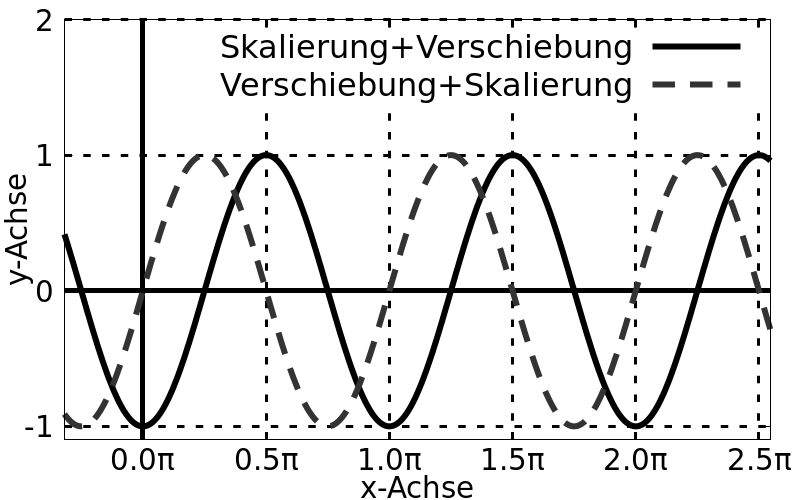
\includegraphics[width=0.95\textwidth]{../tex-snippets/ex-fn-transform-4-a.png}
\end{center}

\begin{enumerate}
\item Erst Skalierung, dann Verschiebung: $g(x) = \cos\left(2(x-\frac{\pi}{2}\right)$
\item Erst Verschiebung, dann Skalierung: $g(x) = \cos\left(2x-\frac{\pi}{2}\right)$
\end{enumerate}
